\documentclass[10pt,twocolumn]{article}

\usepackage[margin=0.72in]{geometry}
\usepackage[T1]{fontenc}
\usepackage[utf8]{inputenc}
\usepackage{lmodern}
\usepackage{microtype}
\usepackage{graphicx}
\usepackage{booktabs}
\usepackage{array}
\usepackage{tabularx}
\usepackage{amsmath}
\usepackage{enumitem}
\usepackage{xspace}
\usepackage{hyperref}
\usepackage{natbib}

\hypersetup{
  colorlinks=true,
  linkcolor=blue,
  citecolor=blue,
  urlcolor=blue
}

\setlist[itemize]{leftmargin=1.1em, itemsep=1.5pt, topsep=2pt}
\setlist[enumerate]{leftmargin=1.2em, itemsep=1.5pt, topsep=2pt}
\setlength{\textfloatsep}{6pt plus 1pt minus 2pt}
\setlength{\floatsep}{6pt plus 1pt minus 2pt}
\setlength{\intextsep}{6pt plus 1pt minus 2pt}
\setlength{\abovecaptionskip}{4pt}
\setlength{\belowcaptionskip}{0pt}

\newcommand{\system}{KernelTuner\xspace}
\newcommand{\artifact}[1]{\texttt{#1}}

\title{Matched-Budget Triton Tuning: Cheap Signals, Realistic Workloads, and Bounded Recovery}
\author{Project Draft}
\date{April 2026}

\begin{document}
\maketitle

\begin{abstract}
The practical question in Triton tuning is not whether search can find good schedules, but what a small measurement budget can buy. This paper studies that question under matched budget: can cheap compile-adjacent signals and bounded profiling guide schedule selection better than default settings or equally budgeted naive baselines? We evaluate a fixed-kernel tuning framework on a homogeneous RTX A6000 pool using representative and aligned GEMM workloads plus regime-split LayerNorm. The main findings are that compile-adjacent signals prune better than they rank, aligned GEMM materially overstates selector quality, profiling is kernel- and regime-dependent rather than uniformly helpful, and transfer failures provide useful evidence for retiring unstable knob families. On the final non-\texttt{split\_k} GEMM surface, a conservative selector reaches 1.0286 geometric-mean speedup versus default, compared with 0.8101 for the compile-ranked parent and 1.0011 for naive random search under the same matched budget. The result is intentionally bounded rather than universal. The paper's contribution is therefore not a claim that Triton tuning is solved, but a clearer empirical account of what lightweight evidence can and cannot buy once the budget and workload realism are fixed.
\end{abstract}

\section{Introduction}

What counts as a win in kernel tuning changes once the search budget is fixed and the workloads are realistic. A selector that looks strong on aligned shapes or after an unstable transfer trick is not necessarily useful in practice. This paper takes that constraint seriously. Rather than asking whether Triton autotuning can ever find a fast schedule, it asks whether a small, explicit evidence budget can be spent better than default settings or equally budgeted naive baselines.

That framing matters because the final positive result in this project is modest. The paper would be weak if it relied only on a single speedup number. Its strength comes from a broader lesson: cheap signals help, but mostly as pruning evidence; realistic workloads expose failures that convenience cases can hide; profiling is mixed rather than uniformly beneficial; and negative transfer results are useful because they justify a cleaner final mainline surface. The final representative-GEMM improvement is worth reporting because it survives those harsher tests, not because it overwhelms them.

\section{Background and Context}

Triton makes schedule-oriented GPU programming practical, but it does not remove the tuning problem. A single kernel still exposes tile sizes, grouped launch order, warp count, and pipeline depth choices whose best setting depends on workload geometry and hardware bottlenecks. Exhaustive autotuning can recover good schedules, but it is often too expensive to treat as the default workflow. That makes matched-budget tuning important: if only a small amount of benchmarking and profiling is affordable, which evidence is worth paying for?

This is also a workload-design problem. On regular aligned shapes, a selector can look stronger than it really is. On irregular representative shapes, ranking failures appear that aligned cases smooth over. Likewise, profiling may help on one kernel or regime and add little on another. A useful paper in this setting must therefore explain not only whether a selector wins, but also what kind of evidence is responsible for the result and why the result changes across workloads.

The paper is narrower than compiler-scale autoscheduling on purpose. It keeps the Triton kernel fixed, studies only bounded schedule knobs, and asks what can be justified under the same budget for every competing strategy. That narrower scope is what makes the negative results interpretable rather than incidental.

\section{Goal}

The goal of this project is to test whether a bottleneck-aware, schedule-first selector can spend a small fixed measurement budget better than default settings or naive baselines for Triton kernels. The paper focuses on three concrete questions:
\begin{itemize}
\item Do cheap compile-adjacent signals do enough to rank good schedules, or do they mainly prune bad ones?
\item Do realistic workloads change the apparent quality of a selector?
\item Can limited profiling and conservative selector refinement recover a credible positive result without hiding failures?
\end{itemize}

\section{Prior Work}

The broad conceptual lineage comes from schedule search and autoscheduling in systems such as Halide, TVM, Ansor, TensorIR, and MetaSchedule \citep{ragankelley2012halide,mullapudi2016halide,adams2019halide,chen2018tvm,zheng2020ansor,zheng2022tensorir,shao2022metaschedule}. Triton itself provides local autotuning interfaces, and PyTorch increasingly treats Triton as part of a larger compilation stack \citep{tillet2019triton,openai2021triton,tritondocsautotune,tritondocsheuristics,pytorchcompile2026,pytorchtriton2026}. External autotuners such as Kernel Tuner, CLTune, and KTT are even closer in spirit because they treat kernels as parameterized programs and compare search strategies directly \citep{vanwerkhoven2019kerneltuner,nugteren2015cltune,petrov2023ktt}. Recent agentic GPU optimization work is broader still, targeting full-kernel generation rather than bounded schedule selection \citep{dai2026cudaagent}.

What is less well covered by prior work is the narrow middle ground this paper targets: fixed Triton kernels, explicit matched-budget comparisons, reportable versus diagnostic profiling, and a willingness to preserve negative results. That narrower question is not larger than prior autotuning systems, but it is scientifically cleaner for understanding what lightweight evidence actually buys.

\begin{table}[t]
\centering
\small
\begin{tabular}{p{0.28\columnwidth}p{0.60\columnwidth}}
\toprule
System family & Relation to this paper \\
\midrule
Halide / TVM-style autoscheduling & Broader schedule languages and compiler objectives than this fixed-kernel study \\
Triton-native autotuning & Immediate ecosystem context; this paper asks what lightweight evidence buys before broad local search \\
External kernel autotuners & Closest practical baseline family; this paper adds stricter matched-budget and evidence rules \\
Agentic GPU optimization & Useful contrast, but much broader than bounded Triton schedule selection \\
\bottomrule
\end{tabular}
\caption{This paper occupies a middle ground: narrower than compiler-scale or agentic optimization, but more controlled than a simple benchmark-driven tuning script.}
\label{tab:condensed-positioning}
\end{table}

\section{Methodology}

All primary studies used by the final paper use a homogeneous RTX A6000 pool across \texttt{gpunode2} and \texttt{gpunode3}. Representative GEMM is the truth source, aligned GEMM is supporting context, and LayerNorm is a secondary regime-split validation kernel. The kernels themselves stay fixed; only bounded schedule knobs change.

Every comparison is budget matched. The main selector ladder is \texttt{default\_config}, \texttt{naive\_random\_search}, compile-ranked \texttt{prune\_rank}, bounded profiling variants, and revised selectors under the same benchmark/profile caps. The canonical reportable representative-GEMM program uses a bounded non-\texttt{split\_k} surface with 216 valid configurations and a matched budget of 12 benchmarks and 4 profiles. Repeatability uses repeated runs with a fixed seed, while robustness uses one run each at seeds 7, 19, and 43. Diagnostic runs may explain a failure, but they are never treated as superiority evidence by themselves.

The evaluation also separates calibration from held-out testing. Strategies may spend their limited budget on calibration shapes, but the headline comparison is always taken from held-out workloads. That distinction matters because the paper is not asking who can overfit a tiny calibration set; it is asking whether the evidence ladder generalizes to representative workloads under the same spend.

\begin{table}[t]
\centering
\small
\begin{tabular}{p{0.29\columnwidth}p{0.58\columnwidth}}
\toprule
Item & Final study choice \\
\midrule
Primary truth source & Representative GEMM \\
Context workload & Aligned GEMM \\
Secondary kernel & LayerNorm, split into \texttt{small\_batch} and \texttt{large\_batch} \\
Canonical GEMM budget & 12 benchmarks, 4 profiles \\
Mainline GEMM surface & non-\texttt{split\_k}, 216 valid configurations \\
Reportable evidence & Held-out runtime plus bounded reportable profiling \\
\bottomrule
\end{tabular}
\caption{Compact study scope for the condensed paper. The work is narrow on purpose: fixed kernels, bounded schedules, explicit budgets, and one primary truth source.}
\label{tab:condensed-scope}
\end{table}

\section{Observations and Motivation}

The first observation is that compile-adjacent signals are useful for pruning but not sufficient for final ranking. On the expanded Phase 2 representative GEMM surface, \texttt{naive\_random\_search} reaches 1.0331 geometric-mean speedup versus default, while the compile-ranked parent \texttt{prune\_rank} reaches only 0.8265. Even bounded profiling helps only modestly at 0.8444. The issue is therefore not whether cheap signals help at all; it is that they cannot reliably separate several already-plausible families.

The second observation is that workload realism changes the conclusion. Figure~\ref{fig:condensed-aligned} shows that aligned GEMM is materially more flattering than representative GEMM. A selector that looks passable on aligned shapes can still be weak on the workload matrix that better reflects realistic irregular cases.

\begin{figure}[t]
\centering
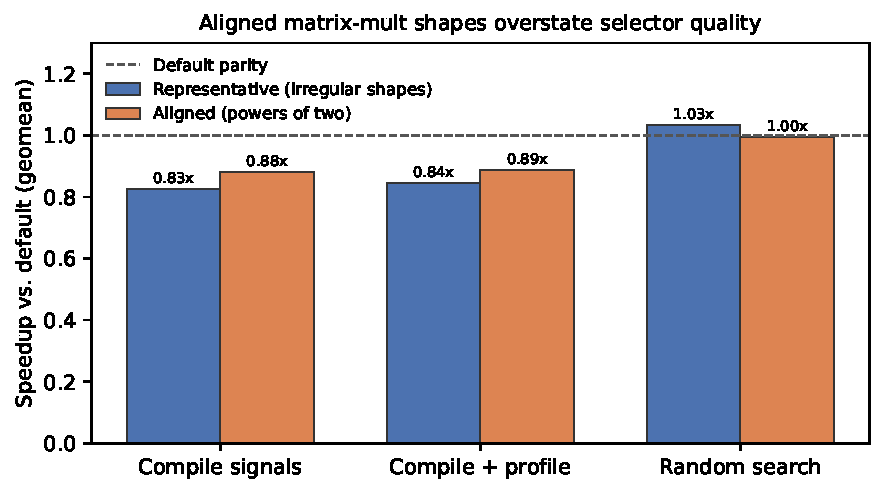
\includegraphics[width=0.98\columnwidth]{figures/generated/figure3_aligned_context.pdf}
\caption{Realistic workloads change the answer. Aligned GEMM makes the selector look stronger than it is on representative GEMM, so aligned results stay contextual rather than headline evidence.}
\label{fig:condensed-aligned}
\end{figure}

LayerNorm adds a third motivation. It does not become a second optimization story; instead, it shows that profiling is regime-dependent. Small-batch behavior is weak and noisy, while large-batch behavior remains negative relative to compile-only ranking. That mixed result makes the broader narrative more believable.

Together, these observations shift the paper away from a simple ``did the selector win'' framing. The more important question becomes which parts of the evidence ladder remain trustworthy once the workload program is made harder and the search surface is allowed to fail.

\section{Ideas and Solutions}

The project responded to these observations by tightening the evidence hierarchy instead of opening a larger heuristic space. Compile-adjacent signals are used first, profiling is bounded and treated separately from diagnostic evidence, and selector revisions are compared only against matched-budget parents. When the expanded Phase 3 \texttt{split\_k} surface failed badly, the paper did not stretch the claim to keep that knob alive. It used the failure to retire \texttt{split\_k} from the mainline GEMM surface and to retire \texttt{rows\_per\_program} from the mainline LayerNorm surface.

The final positive push is therefore conservative by design. The \texttt{v5} selector does not introduce another broad revision family. It corrects frontier construction on the final non-\texttt{split\_k} GEMM surface and applies profiling only within that guarded frontier. The scientific point is not that one more heuristic solved the problem. It is that bounded corrective action can still recover a useful headline once the transfer failures are understood.

\section{Results}

The evidence ultimately resolves into four short answers. First, cheap signals prune but do not rank. That is the most stable primary lesson and the one that best survives the broader non-\texttt{split\_k} Phase 2 space.

Second, realistic workloads matter. Aligned GEMM remains useful because it demonstrates how much better the selector can look on easier shapes than on the representative workload program.

Third, LayerNorm stays regime-split and secondary. In Phase 2, \texttt{small\_batch} moves only from \texttt{prune\_rank}=1.0100 to \texttt{prune\_rank\_profiled}=1.0113, while \texttt{large\_batch} moves the wrong way, from 1.0029 to 0.9856. The later microstudy does not rescue that story; it only confirms that \texttt{rows\_per\_program} is too weak to keep in the final mainline.

Fourth, transfer failed on \texttt{split\_k}, but bounded recovery remained possible on the final mainline. Phase 3 provides the most important negative result: on the expanded \texttt{split\_k} surface, the transfer-safe revision remains unsupported, with \texttt{prune\_rank}=1.0324, \texttt{naive\_random\_search}=1.0427, and \texttt{v4\_transfer\_safe\_profiled}=0.1609. That is why transfer failure belongs in the main story rather than in an appendix.

\begin{figure}[t]
\centering
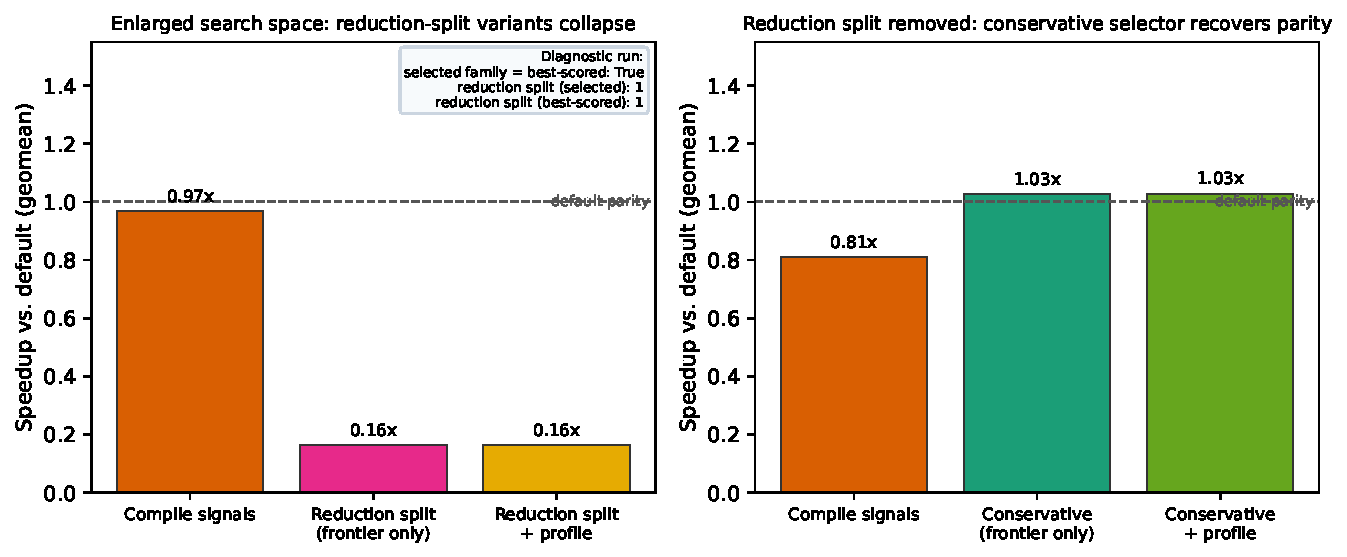
\includegraphics[width=0.98\columnwidth]{figures/generated/figure5_transfer_mainline.pdf}
\caption{Transfer failure is informative, not disposable. The expanded \texttt{split\_k} surface fails badly, but the final non-\texttt{split\_k} mainline still admits a bounded recovery.}
\label{fig:condensed-transfer}
\end{figure}

The final mainline result is positive, but it is intentionally bounded. On representative GEMM, the guarded \texttt{v5\_mainline\_profiled} selector reaches 1.0286 geometric-mean speedup versus default. It also exceeds \texttt{naive\_random\_search}=1.0011 under the same matched budget and clearly beats the compile-ranked parent at 0.8101. The mainline ablation shows that most of this recovery comes from conservative frontier construction, with profiling adding only a small extra increment once the frontier is already correct.

The paper does not strengthen that outcome into a universal success claim. The result is kept at the ``bounded improvement'' tier because the positive mean result is stronger than the seed-level robustness story. That restraint is part of the contribution: the paper only claims what the evidence package clearly supports.

\begin{table}[t]
\centering
\small
\begin{tabular}{p{0.42\columnwidth}r}
\toprule
Strategy & Geomean speedup vs default \\
\midrule
\texttt{prune\_rank} & 0.8101 \\
\texttt{naive\_random\_search} & 1.0011 \\
\texttt{v5\_mainline\_frontier} & 1.0272 \\
\texttt{v5\_mainline\_profiled} & 1.0286 \\
\bottomrule
\end{tabular}
\caption{The final representative-GEMM headline is small but credible: the guarded non-\texttt{split\_k} selector beats the compile-ranked parent and slightly exceeds naive random search under the same matched budget.}
\label{tab:condensed-headline}
\end{table}

Taken together, the evidence makes the project-level interpretation cleaner. `H1` stays strong. `H2` stays mixed and bounded. `H3` remains contextual. `H4` becomes a transfer story rather than a simple success story. `H5` is unsupported on the expanded \texttt{split\_k} surface. The final positive headline matters precisely because it appears after those harsher results rather than instead of them.

\section{Takeaways}

\begin{itemize}
\item Cheap compile-adjacent signals help most as pruning evidence, not as a complete ranking solution.
\item Workload realism changes conclusions materially; aligned GEMM is useful context but not the truth source.
\item Profiling is kernel- and regime-dependent rather than uniformly beneficial.
\item Negative results matter. The Phase 3 \texttt{split\_k} failure justified retiring unstable knob families and made the final mainline result more credible.
\item What worked best in the end was not a larger selector family, but a conservative correction on a better-defined mainline surface.
\end{itemize}

\section{Conclusion}

This paper asked whether matched-budget Triton tuning can do better than defaults or naive baselines using cheap compile-adjacent signals and bounded profiling. The answer is yes, but only in a narrow and carefully evidenced sense. The most useful lesson is not that the final selector is universally strong. It is that lightweight evidence is valuable in specific ways: for pruning, for exposing workload realism, for showing when profiling helps only conditionally, and for justifying why some schedule families should be retired. Within that disciplined framing, the final non-\texttt{split\_k} selector delivers a small but credible representative-GEMM improvement that is worth reporting precisely because the paper also preserves the limits of the method.

That is the strongest way to read the project as a paper. The final selector matters, but the more durable contribution is the empirical template around it: matched-budget comparisons, realistic workload design, regime-aware interpretation, and a willingness to keep transfer failures in the main story. Those choices turn a modest final speedup into a more convincing systems result.

\bibliographystyle{plainnat}
\bibliography{refs}

\end{document}
